\documentclass[12pt]{article}

\setlength{\topmargin} {-1in}

% Style modifications
\oddsidemargin  0.25in
\evensidemargin 0.25in
\textwidth      6.0in
%\textheight     8.0in
%\textheight     8.5in % Changed on 13 September 2012
\textheight     9in % Changed on 3 October 2013
\parskip        0.1in
\parindent      0.0in
\headheight     1.0in

\headsep        .25in


%\pagestyle      {headings}

% Packages
\usepackage{graphicx}
\usepackage{amsmath,amsfonts,amssymb,amscd,verbatim,graphicx,fancyhdr,tikz}
\usepackage{circuitikz}
\usepackage{mathtools} %for minus plus sign alignment in matrices and vectors, added 13 Feb 2017
\usepackage{pgfplots}
\usetikzlibrary{arrows,automata}
\usetikzlibrary{positioning}
\usepgfplotslibrary{groupplots}
\pgfplotsset{compat=1.16}

\usepackage{palatino}
%\usepackage{cmbright}
\usepackage{enumerate}
\usepackage{multicol}
\usepackage{listings}
\usepackage{color}
\usepackage{float}
\usepackage{esdiff} % Derivatives
\usepackage{cleveref}
\usepackage{siunitx}
\usepackage{caption}
\usepackage{subcaption}
\usepackage[ruled,vlined]{algorithm2e}

\usepackage{tikz} %Can be used to draw Markov Chains or other Graphs
% See http://www.freeminded.org/index.php/2010/05/a-markov-chain-in-tikz/
\usetikzlibrary{arrows.meta}

\newcommand\eqnnumber{\addtocounter{equation}{1}\tag{\theequation}} % Allows us to tag the last equation in an align


%The accents package is included so I can type bold dots for time derivatives
\usepackage{accents}
\newcommand*{\dt}[1]{%
\accentset{\mbox{\large\bfseries .}}{#1}}
\newcommand*{\ddt}[1]{%
\accentset{\mbox{\large\bfseries .\hspace{-0.25ex}.}}{#1}}



%%% Some Mathematical Environmental Definitions
\newcommand{\reals}{{\rm Reals}}
\newcommand{\B}[1]{\mathbf{#1}}
% the following line was added for the vector bold.
\DeclareMathAlphabet{\V}{OML}{cmm}{b}{it}
% Since the above gives a strange looking bold 0 (zero) we do this:
% (To be used only in math mode)
%\newcommand{\0}{\mbox{\bf 0}}
\newcommand{\bs}[1]{\boldsymbol{#1}}
\newcommand{\underscore}{\char`\_}
\newcommand{\tildetext}{\char`\~}
\newcommand{\defn}{\stackrel{\triangle}{=}}
\newcommand{\cas}{\text{cas }}

\newcommand{\var}{\textup{var}}
\def\P{{\bf P}}
\def\E{{\bf E}}
\newcommand{\cov}{\textup{cov}}

\def\E{{\bf E}}
\def\P{{\bf P}}
\def\var{\text{var}}
\def\cov{\text{cov}}
\def\e{\mathrm{e}}

\DeclareMathOperator*{\argmin}{argmin}
\DeclareMathOperator*{\argmax}{argmax}

\Crefname{algocf}{Algorithm}{Algorithms}

%%% ENTER COURSE NUMBER AND NAME HERE
\newcommand{\coursenumber}{EECS~16ML}
\newcommand{\coursename}{Practical Machine Learning}
\newcommand{\coursetitle}{\coursenumber: \coursename}
\newcommand{\docauthor}{Anmol Parande}

%%% WHAT KIND OF DOCUMENT IS THIS?
\newcommand{\documenttype}{note} % Other examples: exam, quiz, final, midterm, homework
\newcommand{\titledocumenttype}{Note} % This is what appears in the document header

% What is the document number? e.g., 5, if this is homework 5, or quiz 5, ...
\newcommand{\documentnumber}{1}

%%% Problem Prefix, e.g., HW1, or MT2, or F1
\newcommand{\pp}{\documentinitials\documentnumber}

%%% Document Headers
\lhead{{\coursetitle} \\ \titledocumenttype \mbox{} \documentnumber \\ [-10pt]}
\rhead{Fall 2020 \\ [-10pt]}



% What is the document number? e.g., 5, if this is homework 5, or quiz 5, ...
\renewcommand{\documentnumber}{x}

\begin{document}
  \thispagestyle{fancy}
  \newpage

  In EECS 16A, you saw the OMP algorithm as a method to find a sparse set of circularly-shifted vectors whose linear combination constituted a received signal.
  The motivation was in the context of decoding messages sent from satellites. It turns out that that this idea of finding a sparse-linear combination can also help us in Machine Learning. In particular it helps us with the problem of outlier removal.
  \section{Recap of OMP}
  Before we see how OMP is used in Machine Learning, let's do a brief recap of the algorithm by returning to the context in which EECS 16A covered it. 
  Suppose we have $m$ satellites, each periodically transmitting a unique code $\B{s_i}\in\mathbb{R}^n$. 
  Satellites encode messages by multiplying the code they transmit by some scalar $\alpha_i\in\mathbb{R}$.
  At any given moment, only $k$ satellites are transmitting, so at the receiver, we measure the signal
  \[
	\V{y} = \sum_{i\in K} \alpha_i\V{s_i}^{(\tau_i)}
  \]
  where $\tau_i$ is a circular shift induced by the fact that each satellite is some distance away from the receiver and $K$ is the set of all transmitting satellites.
  We need to find out which satellites are transmitting as well as the corresponding messages.
  One natural way to proceed is iteratively. We can first ``predict'' which satellites are transmitting by finding the code $\V{s_i}$ and shift $\tau_k$ such that $\V{s_i}^{(\tau_k)}$ has the largest absolute cross-correlation than any other $\V{s_j}^{(\tau_p)}$ ($i, j \leq m$ and $k, p \leq n$).
  Then, we perform OLS to find the coefficient $\alpha_i$ of $\V{s_i}^{(\tau_k)}$, giving us how much $\V{s_i}^{\tau_k}$ ``explains'' our received signal.
  Finally, we compute the residual $\V{e} = \V{y} - \alpha_i\V{s_i}^{(\tau_k)}$, which tells us how much of our signal we still need to explain, and repeat the process on the residual $k-1$ times (or until our residual is small).
  Each time we repeat, we recompute the $\alpha_i$ since finding more of the satellites will give us a different estimate of $\alpha_i$ each time.
  This process is summarized by \cref{code:omp-16a}.
  \begin{algorithm}[!h]
	\SetAlgoLined
	\KwIn{Codes $\V{s_i}$, Received signal $\V{y}$, Sparsity $k$, Residual Threshold $\epsilon$}
	\KwOut{The indices of the used codes F, the sent messages $\V{x}$} 
	$\V{e} = \V{y}$, j = 1, A = [], F = $\emptyset$\;
	\While{$j \leq k$ and $||\V{e}|| \geq \epsilon$}{
	  i, t = FindMaxCrossCorrelation()\;
	  $F = F \bigcup \{i\}$\;
	  $A = [A | s_i^{(t)}]$\;
	  $\V{x} = (A^TA)^{-1}A^T\V{y}$\;
	  $\V{e} = \V{y} - A\V{x}$\;
	  j = j + 1\;
	}
	\Return{$F, \V{x}$}
	\caption{OMP Algorithm from 16A}
	\label{code:omp-16a}
  \end{algorithm}
  \section{OMP for Outlier Removal in Linear Regression}
  On its face, the setup for OMP seems entirely different from our Linear Regression setup.
  In Linear Regression, we have $n$ targets $y_i = \V{w}^T\V{x_i}+\epsilon_i$ which are the sum of features $\V{x_i}\in\mathbb{R}^m$ weighted by $\V{w}$ with some noise $\epsilon_i$.
  In matrix form, this is
  \[
	\begin{bmatrix}
	  y_1\\y_2\\\vdots\\y_n
	\end{bmatrix} = \begin{bmatrix}
	  \V{x_1}^T\\\V{x_2}^T\\\vdots\\\V{x_n}^T
	\end{bmatrix}\V{w} + \bs{\epsilon}.
  \]
  It might not be entirely obvious at first, but we can interpret this exactly as an OMP problem by properly deciding what to call our ``message`` and what to call our ``codes``.
  First, let's express the OMP problem in matrix form.
  \[
	\V{y} = \begin{bmatrix}
	  \V{s_1}^{(\tau_1)} & \V{s_2}^{(\tau_2)} & \cdots & \V{s_m}^{(\tau_m)}
	\end{bmatrix}\bs{\alpha}
  \]
  If we ignore the noise in the Machine Learning context and the shifts in the OMP context, clearly our received signal $\V{y}$ can be thought of as our targets, and the sparse message $\bs{\alpha}$ is the weights of the model.
  The codes $\V{s_i}$ are simply the columns of the data matrix (i.e the features of each data point). Notice that we can ignore the shifts $\tau_i$ because there is nothing in Linear Regression which suggests a ''delay``, and the noise in the machine learning context translates to the OMP context naturally because there is no guarantee $\V{y}$ is received perfectly.
  \subsection{Outliers}
  How does this interpretation help us with outlier removal exactly?
  An outlier is a point which lies very far from the true linear model.
  Mathematically, it means for the target $y_i$, $\epsilon_i$ is very large, meaning it is either corrupted by a lot of noise or was generated with a different process than the linear model, so it can't be explained by our linear model.

  Because these points can't be well explained by a linear model, if we were to run OLS on data containing outliers, the outliers would skew the model away from the actual fit because OLS will try and balance minimizing the residual to the outliers against minimizing the residual from all of the uncorrupted data.
  Notice how in \cref{fig:good-fit} where there is only a small amount of noise, the learned model reflects the general trend of the data (all of the residuals are small).
  \begin{figure}[!h]
	\centering
	\begin{subfigure}{0.45\textwidth}
	  \centering
	  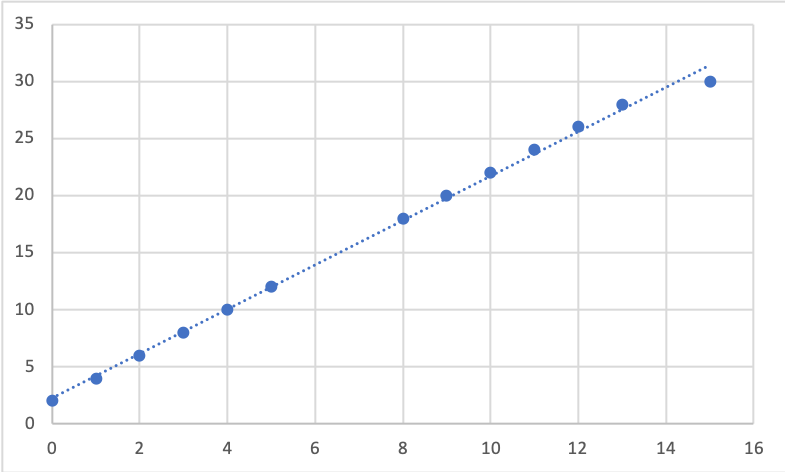
\includegraphics[width=\textwidth]{Images/good_fit}
	  \caption{Model learned without outliers}
	  \label{fig:good-fit}
	\end{subfigure}
	\begin{subfigure}{0.45\textwidth}  
	  \centering
	  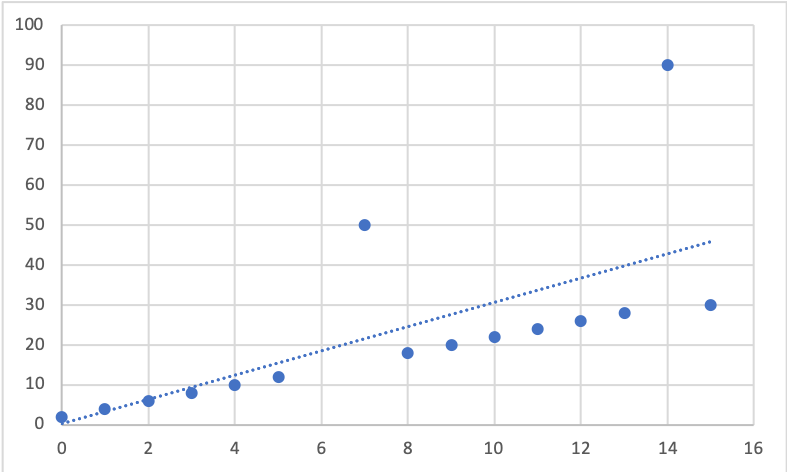
\includegraphics[width=\textwidth]{Images/outlier_fit}
	  \caption{Model learned with outliers}
	  \label{fig:outlier-fit}
	\end{subfigure}
	\caption{}
	\label{fig:different-fits}
  \end{figure}
  However, in \cref{fig:outlier-fit}, the two outliers increase the slope of the line (in an attempt to make the residuals to those two points smaller), decreasing its ability to capture the correct trend.
  \subsection{Interpreting OMP as an Outlier Removal Problem}
  How does OMP help us solve the problem of outliers? Well if we knew which points were outliers, we could remove them from our training set and train with the remaining data.
  Recall that
  \[
	\begin{bmatrix}
	  y_1\\y_2\\\vdots\\y_n
	\end{bmatrix} = \begin{bmatrix}
	  \V{x_1}^T\\\V{x_2}^T\\\vdots\\\V{x_n}^T
	\end{bmatrix}\V{w} + \bs{\epsilon}.
  \]
  If we break up $\bs{\epsilon}$, we see,
  \[
	\begin{bmatrix}
	  y_1\\y_2\\\vdots\\y_n
	\end{bmatrix} = \begin{bmatrix}
	  \V{x_1}^T\\\V{x_2}^T\\\vdots\\\V{x_n}^T
	\end{bmatrix}\V{w} + \sum \epsilon_i \V{e_i} = 
	\begin{bmatrix}
	  X & I
	\end{bmatrix} \begin{bmatrix}
	  \V{w}\\ \bs{\epsilon}
	\end{bmatrix}
  \]
  where $\V{e_i}$ are the standard basis vectors.
  What this tells us is that outliers are essentially large perturbations along the standard basis in feature space.
  Since we only have a few outliers, $\bs{\epsilon}$ is sparse. 

  Thinking about this in the context of OMP, we already know that the features of our data matrix can explain our signal.
  We now need to find the standard basis vectors which also explain our signal.
  In the context of satellites, it is as if we have $m$ satellites transmitting their codes normally but then $k$ ``adversarial'' satellites very loudly transmit one of the standard basis vectors, effectively drowning out the other satellites.
  If we find the loud, ``adversarial'' satellites, then we can remove them and recover our true message again.

  This interpretation naturally leads us to OMP initialized with $A = X$, proceeding as normal thereafter.
  We find the $\V{e_i}$ which most explains our residual, indicating that the ith point is an outlier, augment $A$ with $\V{e_i}$, and continue.
  At the end of the algorithm, we output the set $F$ which tells us the indices of the outliers.
  Once we remove the outliers from the data set, we can proceed as normal with OLS.

  Note that because there are no delays, we don't need to compute the circular cross-correlation. 
  We only need to find the maximum, absolute dot product of each standard basis vector with the residual $\V{r}$. In other words, we need to find
  \[
	i = \argmax_{i} |\langle \V{r}, \V{e_i} \rangle| = \argmax_{i}|\V{r}[i]|
  \]
  where $r[i]$ is the residual for the ith datapoint.
  \begin{algorithm}[!h]	
	\SetAlgoLined
	\KwIn{Data matrix $X$, Predictions $\V{y}$, Sparsity $k$, Residual Threshold $\epsilon$}
	\KwOut{Set of data indices $F$ where the outliers are}
	$\V{r} = \V{y} - X(X^TX)^{-1}X^T\V{y}$, j = 1, A = X, F = $\emptyset$\;
	\While{$j \leq k$ and $||\V{r}|| \geq \epsilon$}{
	  i = $\argmax_i |\V{r}[i]|$\;
	  $F = F \bigcup \{i\}$\;
	  $A = [A | \V{e_i}]$\;
	  $\V{x} = (A^TA)^{-1}A^T\V{y}$\;
	  $\V{r} = \V{y} - A\V{x}$\;
	  j = j + 1\;
	}
	\Return{F}
	\caption{OMP to Detect Outliers}
	\label{code:omp}
  \end{algorithm}

  It turns out that we do not have to initialize OMP with the data matrix $X$. Remember that OMP is selecting the features which best explain our data, so ideally, our actual features should be the ones that best explain the data, so OMP will choose them anyway if we run it on the matrix $[X | I]$.
  However, because OMP is greedily looking for the loudest features, it is possible that if the features are not scaled properly, then OMP might not choose some of our true features because they are too ``quite''.
  This is why it is very important that we engineer our features appropriately to make sure this doesn't happen.
  \subsection{Stopping Conditions}
  At this point, you might be asking yourself, ``How do we know how many outliers are in the dataset?'' or ``How do we know when to stop running OMP?''.
  This question has 3 natural answers for linear regression.
  \begin{enumerate}
	\item[\textbf{Choose $\B{k}$}:] If you know the number of outliers is $k$, then you only need to run OMP for $k$ iterations. You might be able to find a good $k$ by visualizing the dataset and seeing which points deviate significantly from a linear relationship.
	\item[\textbf{Choose $\boldsymbol{\epsilon}$}:] You can also stop OMP when the residual gets ``too small''. The value that determines ``too small'' would be determined by looking at your validation error and finding the $\epsilon$ corresponding to the minimum MSE.
	\item[\textbf{Trivial Case}:] If you only have 2 data points (either by running OMP for too many iterations or just because you have a small dataset), then you can always fit a line that perfectly predicts both points since a line is defined by 2 points. If we reached 2 points by running OMP, then we should stop iterating.
  \end{enumerate}
\end{document}
